%%%%%%%%%%%%%%%%%%%%%%%%%%%%%%%%%%%%%
%                                   %
% Compile with XeLaTeX and biber    %
%                                   %
% Questions or comments:            %
%                                   %
% joshua dot mcneill at uga dot edu %
%                                   %
%%%%%%%%%%%%%%%%%%%%%%%%%%%%%%%%%%%%%

\documentclass{beamer}
  % Read in standard preamble (cosmetic stuff)
  %%%%%%%%%%%%%%%%%%%%%%%%%%%%%%%%%%%%%%%%%%%%%%%%%%%%%%%%%%%%%%%%
% This is a standard preamble used in for all slide documents. %
% It basically contains cosmetic settings.                     %
%                                                              %
% Joshua McNeill                                               %
% joshua dot mcneill at uga dot edu                            %
%%%%%%%%%%%%%%%%%%%%%%%%%%%%%%%%%%%%%%%%%%%%%%%%%%%%%%%%%%%%%%%%

% Beamer settings
% \usetheme{Berkeley}
\usetheme{CambridgeUS}
% \usecolortheme{dove}
% \usecolortheme{rose}
\usecolortheme{seagull}
\usefonttheme{professionalfonts}
\usefonttheme{serif}
\setbeamertemplate{bibliography item}{}

% Packages and settings
\usepackage{fontspec}
  \setmainfont{Charis SIL}
\usepackage{hyperref}
  \hypersetup{colorlinks=true,
              allcolors=blue}
\usepackage{graphicx}
  \graphicspath{{../../figures/}}
\usepackage[normalem]{ulem}
\usepackage{enumerate}

% Document information
\author{M. McNeill}
\title[FREN2001]{Français 2001}
\institute{\url{joshua.mcneill@uga.edu}}
\date{}

%% Custom commands
% Lexical items
\newcommand{\lexi}[1]{\textit{#1}}
% Gloss
\newcommand{\gloss}[1]{`#1'}
\newcommand{\tinygloss}[1]{{\tiny`#1'}}
% Orthographic representations
\newcommand{\orth}[1]{$\langle$#1$\rangle$}
% Utterances (pragmatics)
\newcommand{\uttr}[1]{`#1'}
% Sentences (pragmatics)
\newcommand{\sent}[1]{\textit{#1}}
% Base dir for definitions
\newcommand{\defs}{../definitions}


  % Packages and settings

  % Document information
  \subtitle[Dates]{Les dates importantes}

\begin{document}
  % Read in the standard intro slides (title page and table of contents)
  \begin{frame}
    \titlepage
    \tiny{Office: % Basically a variable for office hours location
Gilbert 121\\
          Office hours: % Basically a variable for office hours
 lundi, mercredi, vendredi 10:10--11:10
}
  \end{frame}

  \begin{frame}{}
    \begin{center}
      \Large Quiz
    \end{center}
  \end{frame}

  \begin{frame}{Les associations}
    Quel nombre est associé avec chaque mot? \\
    \tinygloss{Which number is associated with each word?}
    \begin{columns}
      \column{0.5\textwidth}
        \begin{enumerate}
          \item une paire $\to$ \underline{\uncover<2->{2}}
          \item l'alphabet $\to$ \underline{\uncover<4->{26}}
          \item le premier $\to$ \underline{\uncover<6->{1}}
          \item les mois $\to$ \underline{\uncover<8->{12}}
          \item le vote $\to$ \underline{\uncover<10->{18}}
        \end{enumerate}
      \column{0.5\textwidth}
        \begin{minipage}[c][0.6\textheight]{\linewidth}
          \begin{center}
            \only<1-2>{
              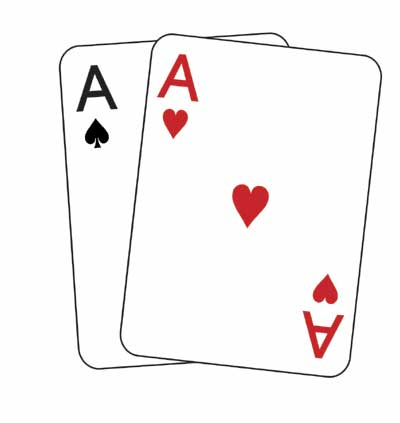
\includegraphics[scale=0.35]{paire.jpg}
            }
            \only<3-4>{
              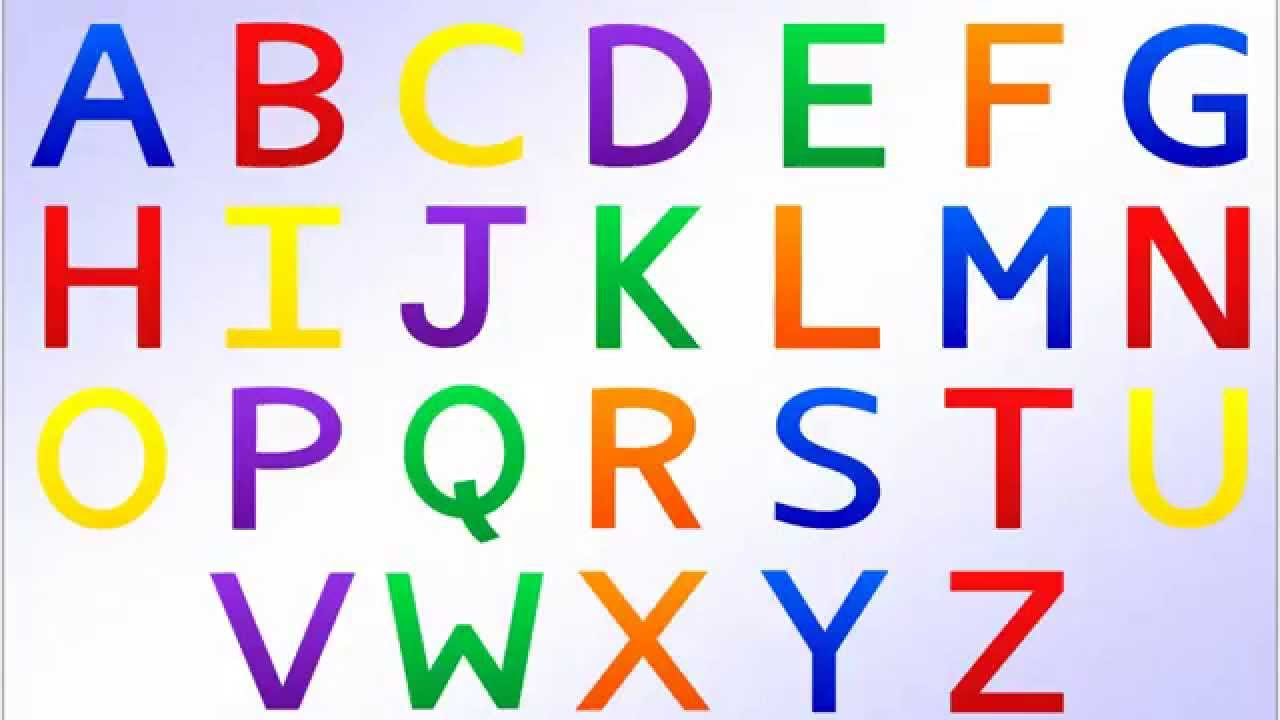
\includegraphics[scale=0.125]{alphabet.jpg}
            }
            \only<7-8>{
              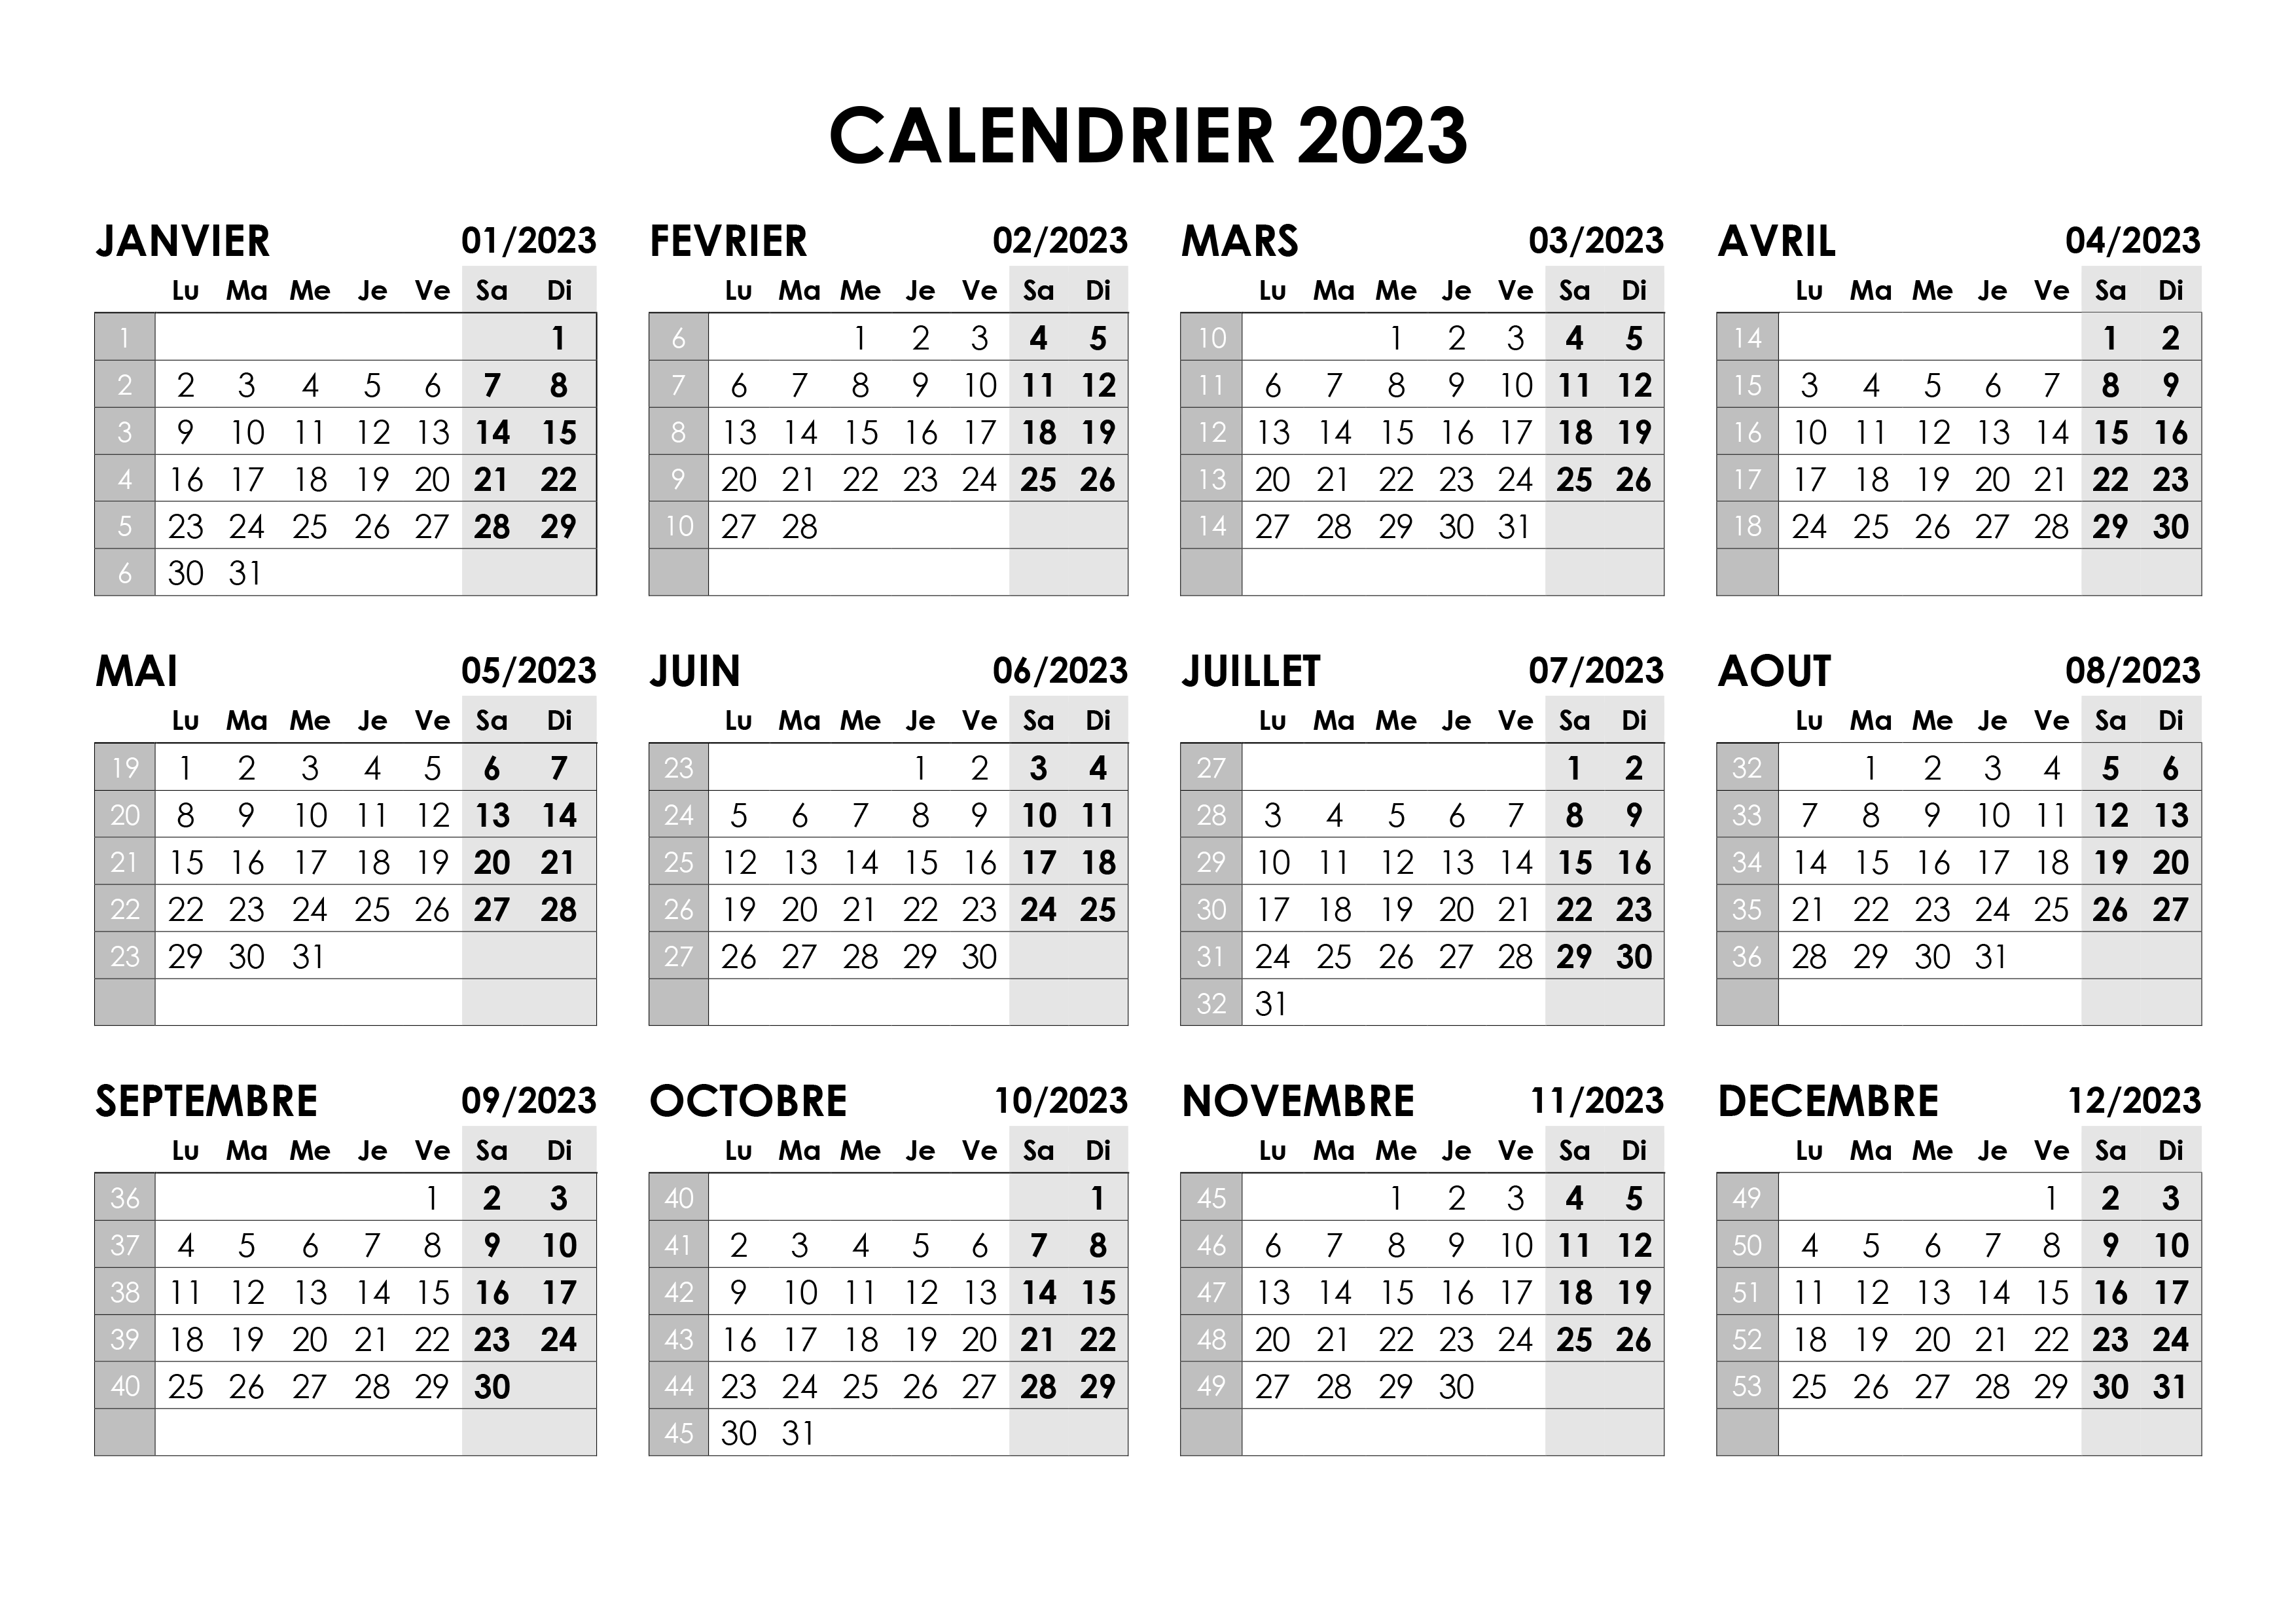
\includegraphics[scale=0.2]{calendrier.png}
            }
            \only<9-10>{
              
\includegraphics[scale=0.25]{vote.png}
            }
          \end{center}
        \end{minipage}
    \end{columns}
  \end{frame}

  \begin{frame}{Les prononciations}
    Quelle est la prononciation? \\
    \tinygloss{What is the pronunciation?}
    \begin{columns}
      \column{0.5\textwidth}
        \begin{enumerate}
          \item cinq\ \ \ filles
          \item cin\textbf<2->{q}\uncover<2->{$_\smile$}enfants
          \item trois\ \ \ frères
          \item troi\textbf<3->{s}\uncover<3->{$_\smile$}oncles
          \item neuf\ \ \ mois
          \item neu\textbf<5->{f}\uncover<5->{$_\smile$}ans
        \end{enumerate}
      \column{0.5\textwidth}
        \begin{minipage}[c][0.6\textheight]{\linewidth}
          \begin{center}
            \only<1-3>{
              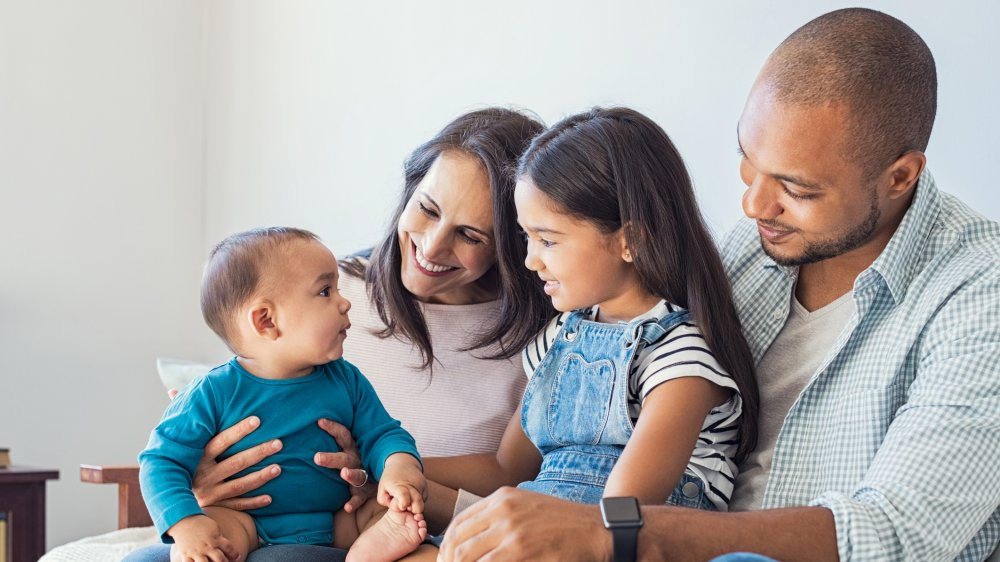
\includegraphics[scale=0.2]{famille_mixte.jpg}
            }
            \only<4->{
              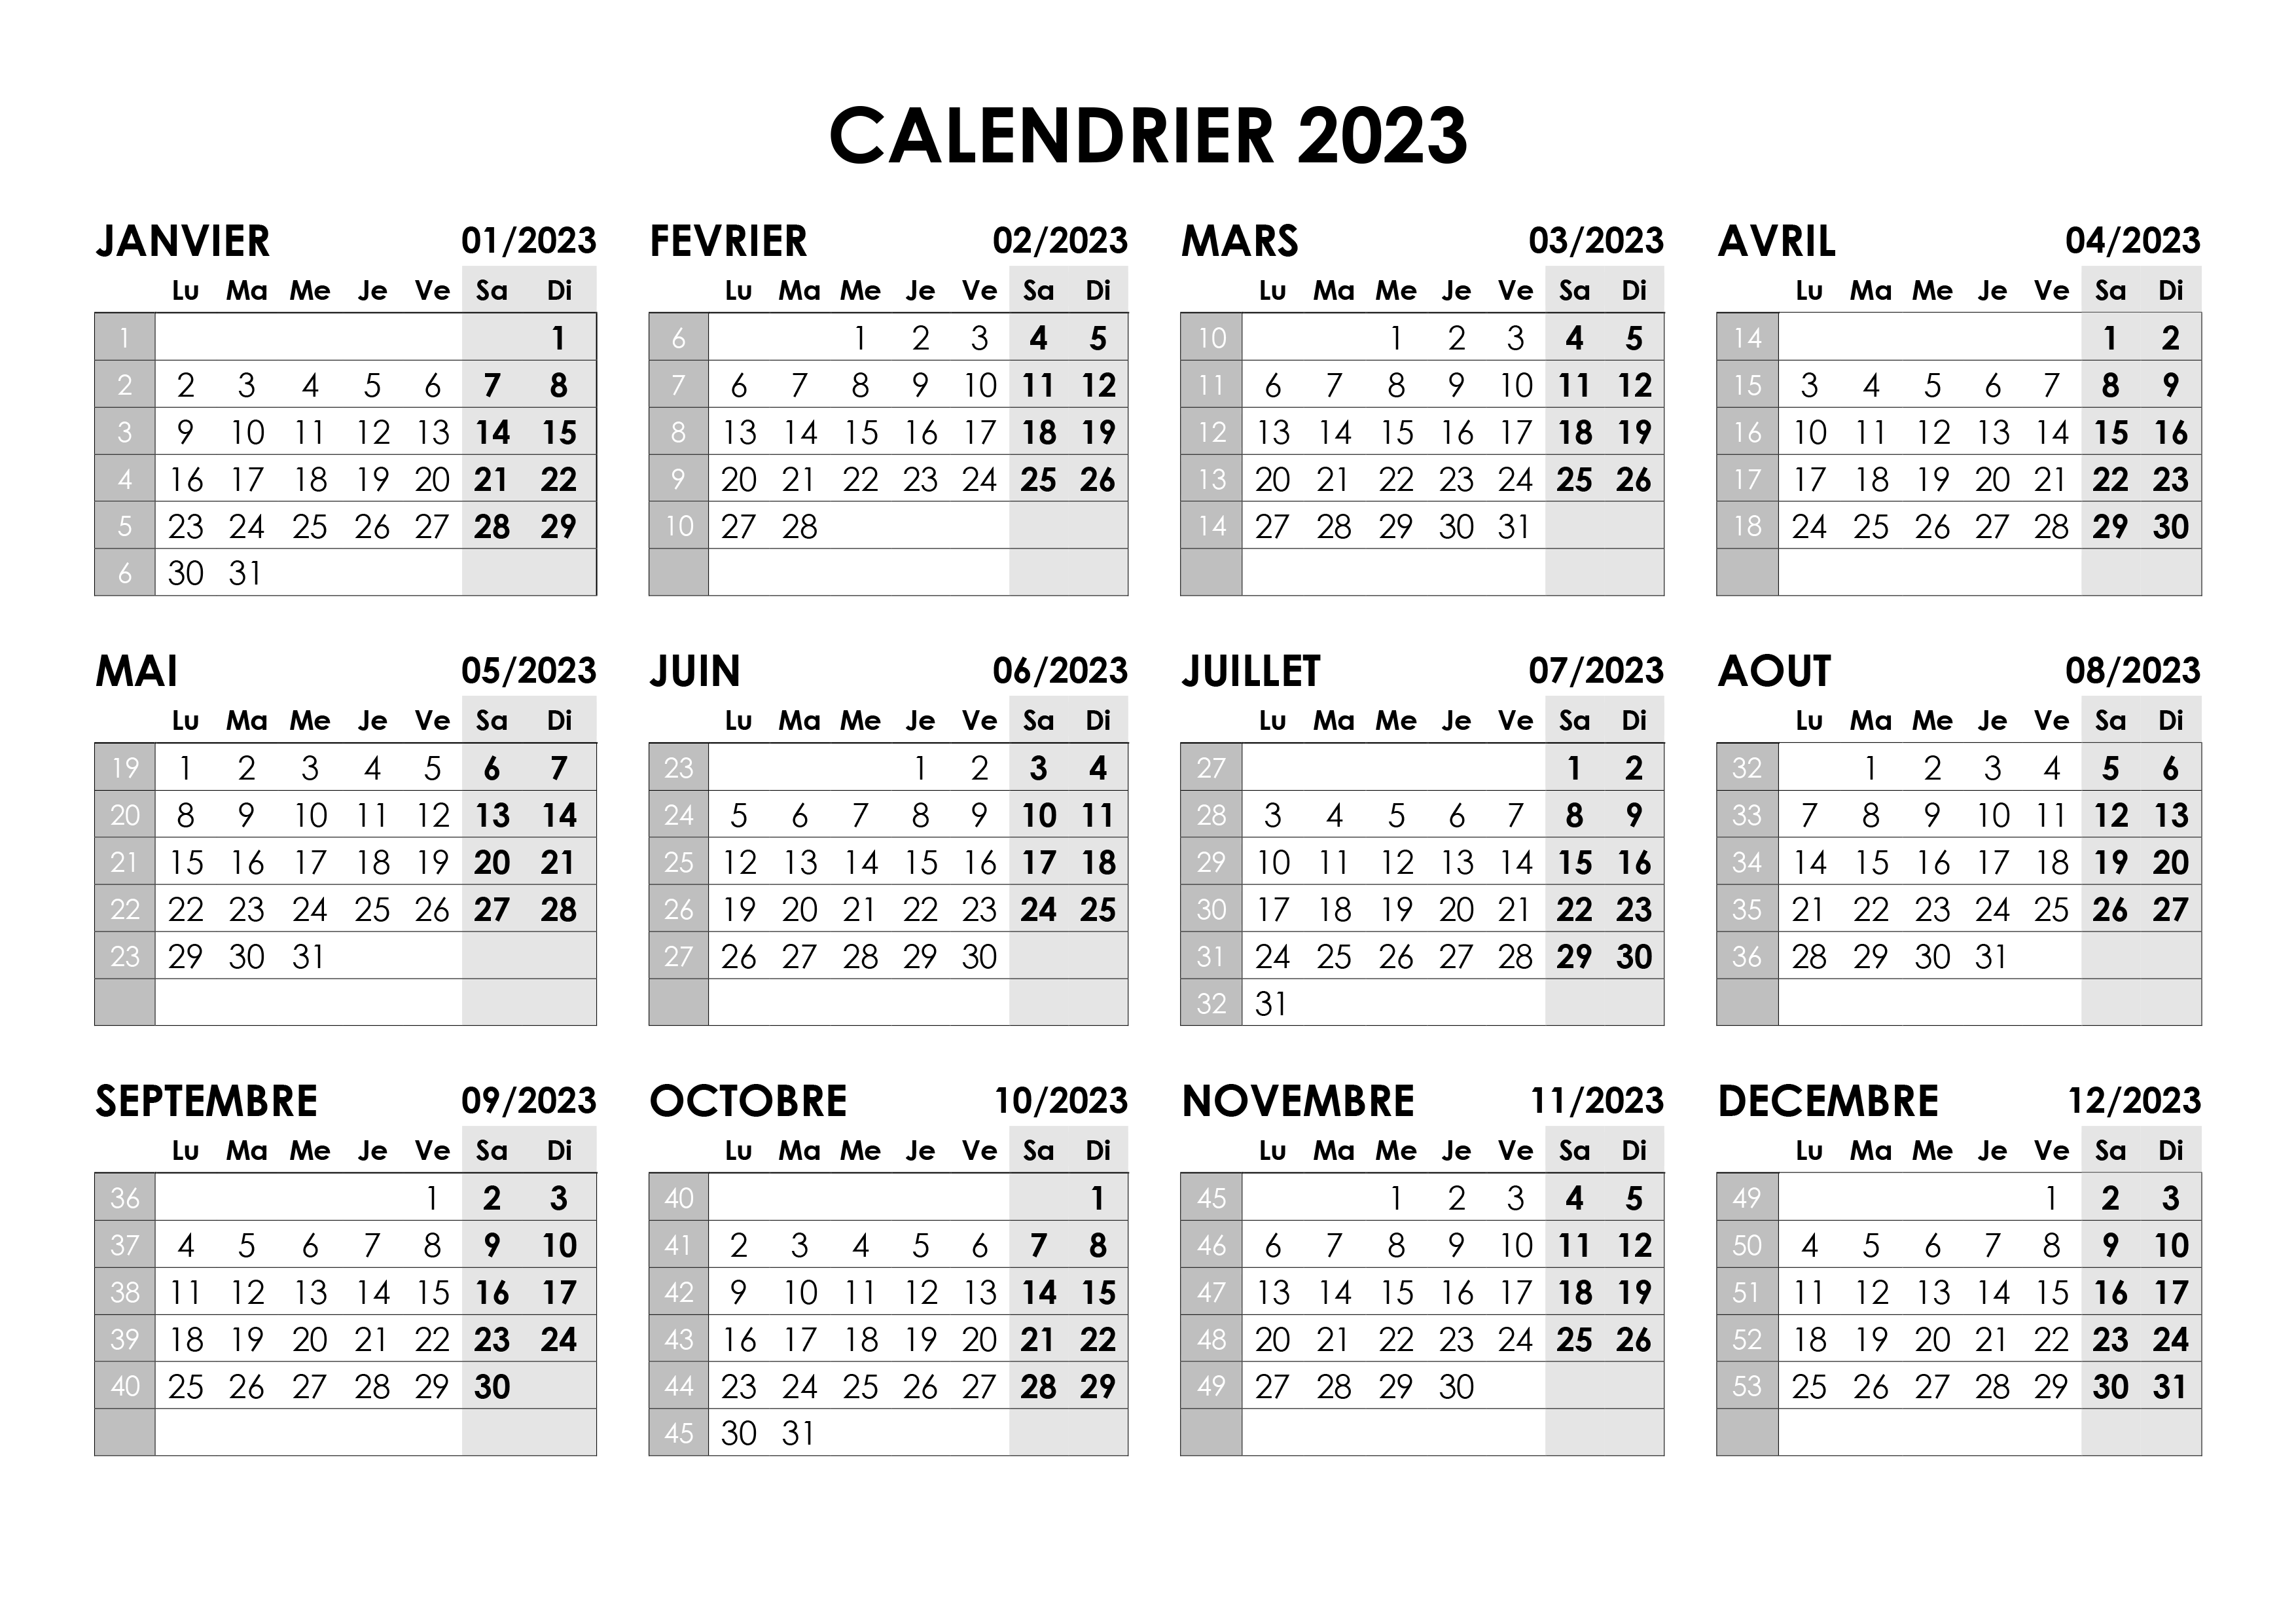
\includegraphics[scale=0.2]{calendrier.png}
            }
          \end{center}
        \end{minipage}
    \end{columns}
  \end{frame}

  \begin{frame}{Les dates}
    Quelle est date aujourd'hui? \underline{\uncover<2->{le 30 août}} \\
    \vspace{0.2cm}
    \uncover<3->{
      Quelle est la date de chaque fête? \\
      \tinygloss{What is the date of each holiday?}
      \begin{columns}
        \column{0.6\textwidth}
          \small
          \begin{enumerate}
            \item le jour de l'An $\to$ \underline{\uncover<4->{le 1er janvier}}
            \item Noël $\to$ \underline{\uncover<6->{le 25 décembre}}
            \item l'indépendance américaine
            \item[$\to$] \underline{\uncover<8->{le 4 juillet}}
            \item le Juneteenth $\to$ \underline{\uncover<10->{le 19 juin}}
            \item la journée des anciens combattants \gloss{veterans}
            \item[$\to$] \underline{\uncover<12->{le 11 novembre}}
          \end{enumerate}
        \column{0.4\textwidth}
          \begin{minipage}[c][0.6\textheight]{\linewidth}
            \begin{center}
              \only<3-4>{
                
\includegraphics[scale=0.16]{nouvel_an.jpg}
              }
              \only<5-6>{
                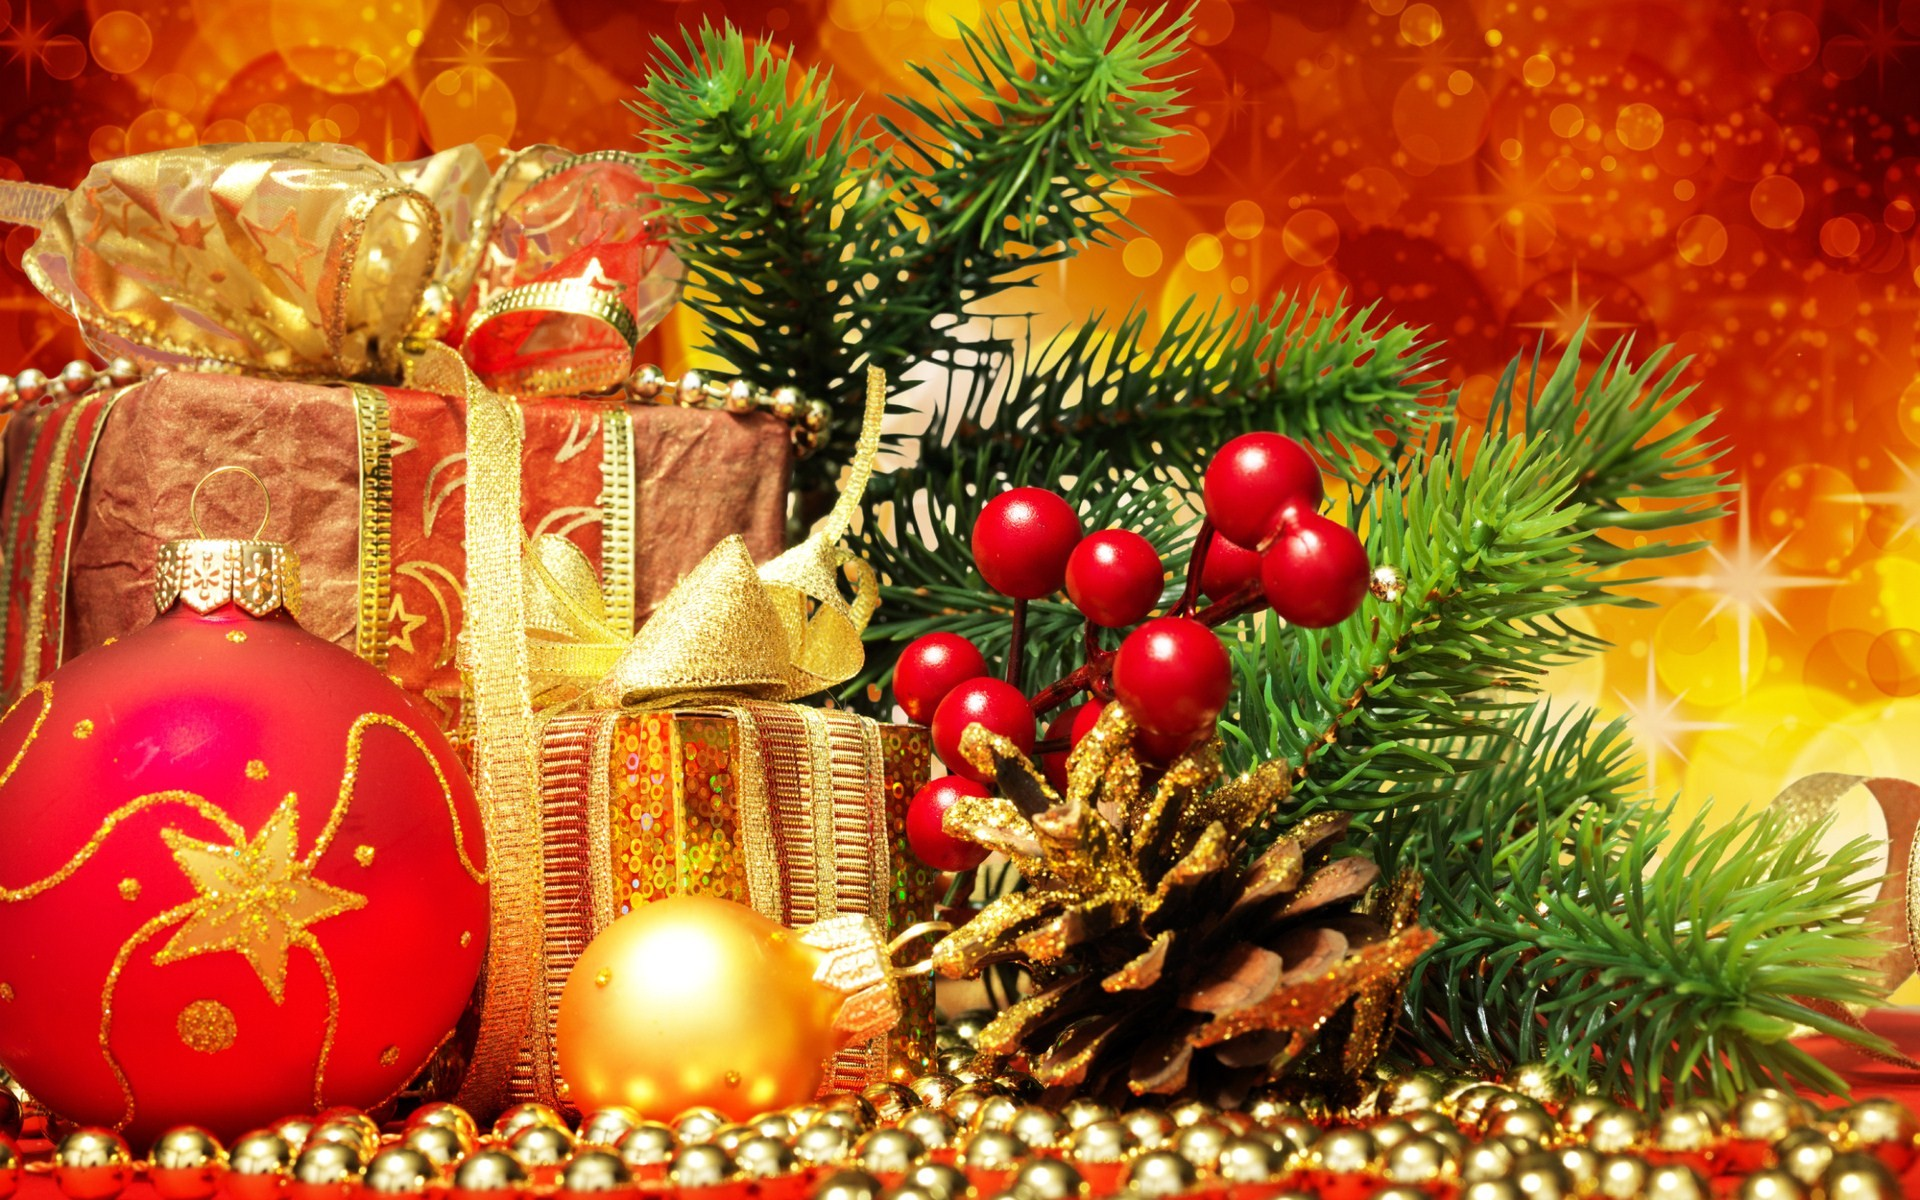
\includegraphics[scale=0.07]{noel.jpg}
              }
              \only<7-8>{
                \includegraphics[scale=0.2]{indépendance.jpg}
              }
              \only<9-10>{
                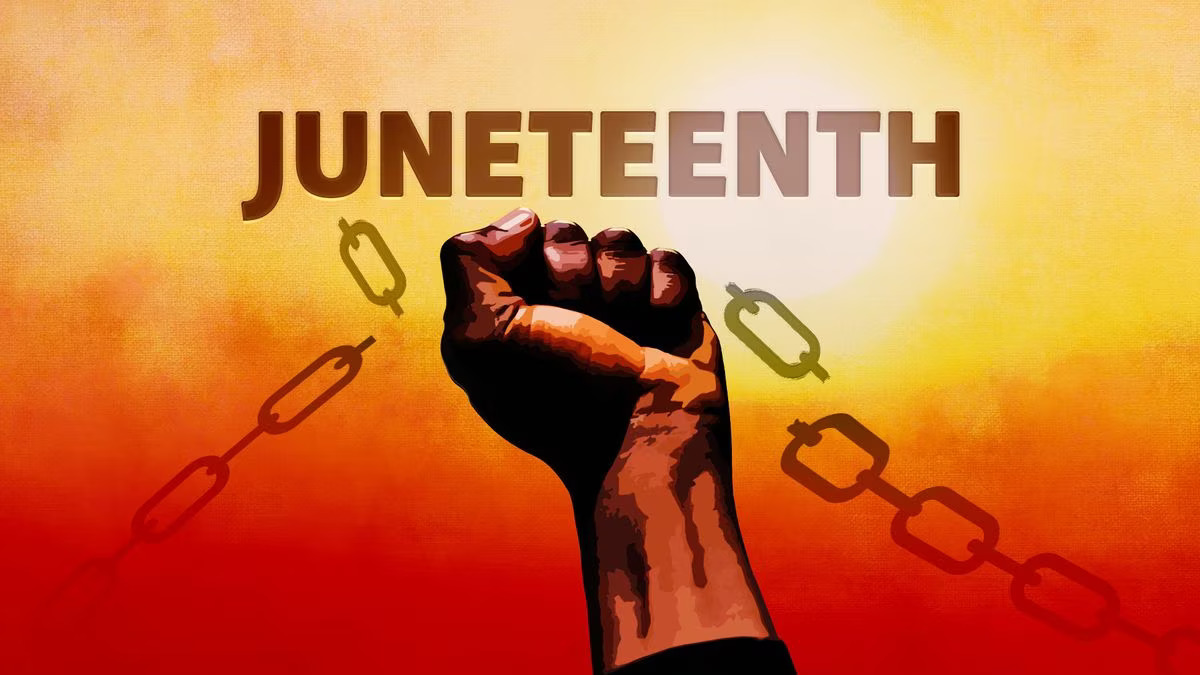
\includegraphics[scale=0.11]{juneteenth.jpg}
              }
              \only<11-12>{
                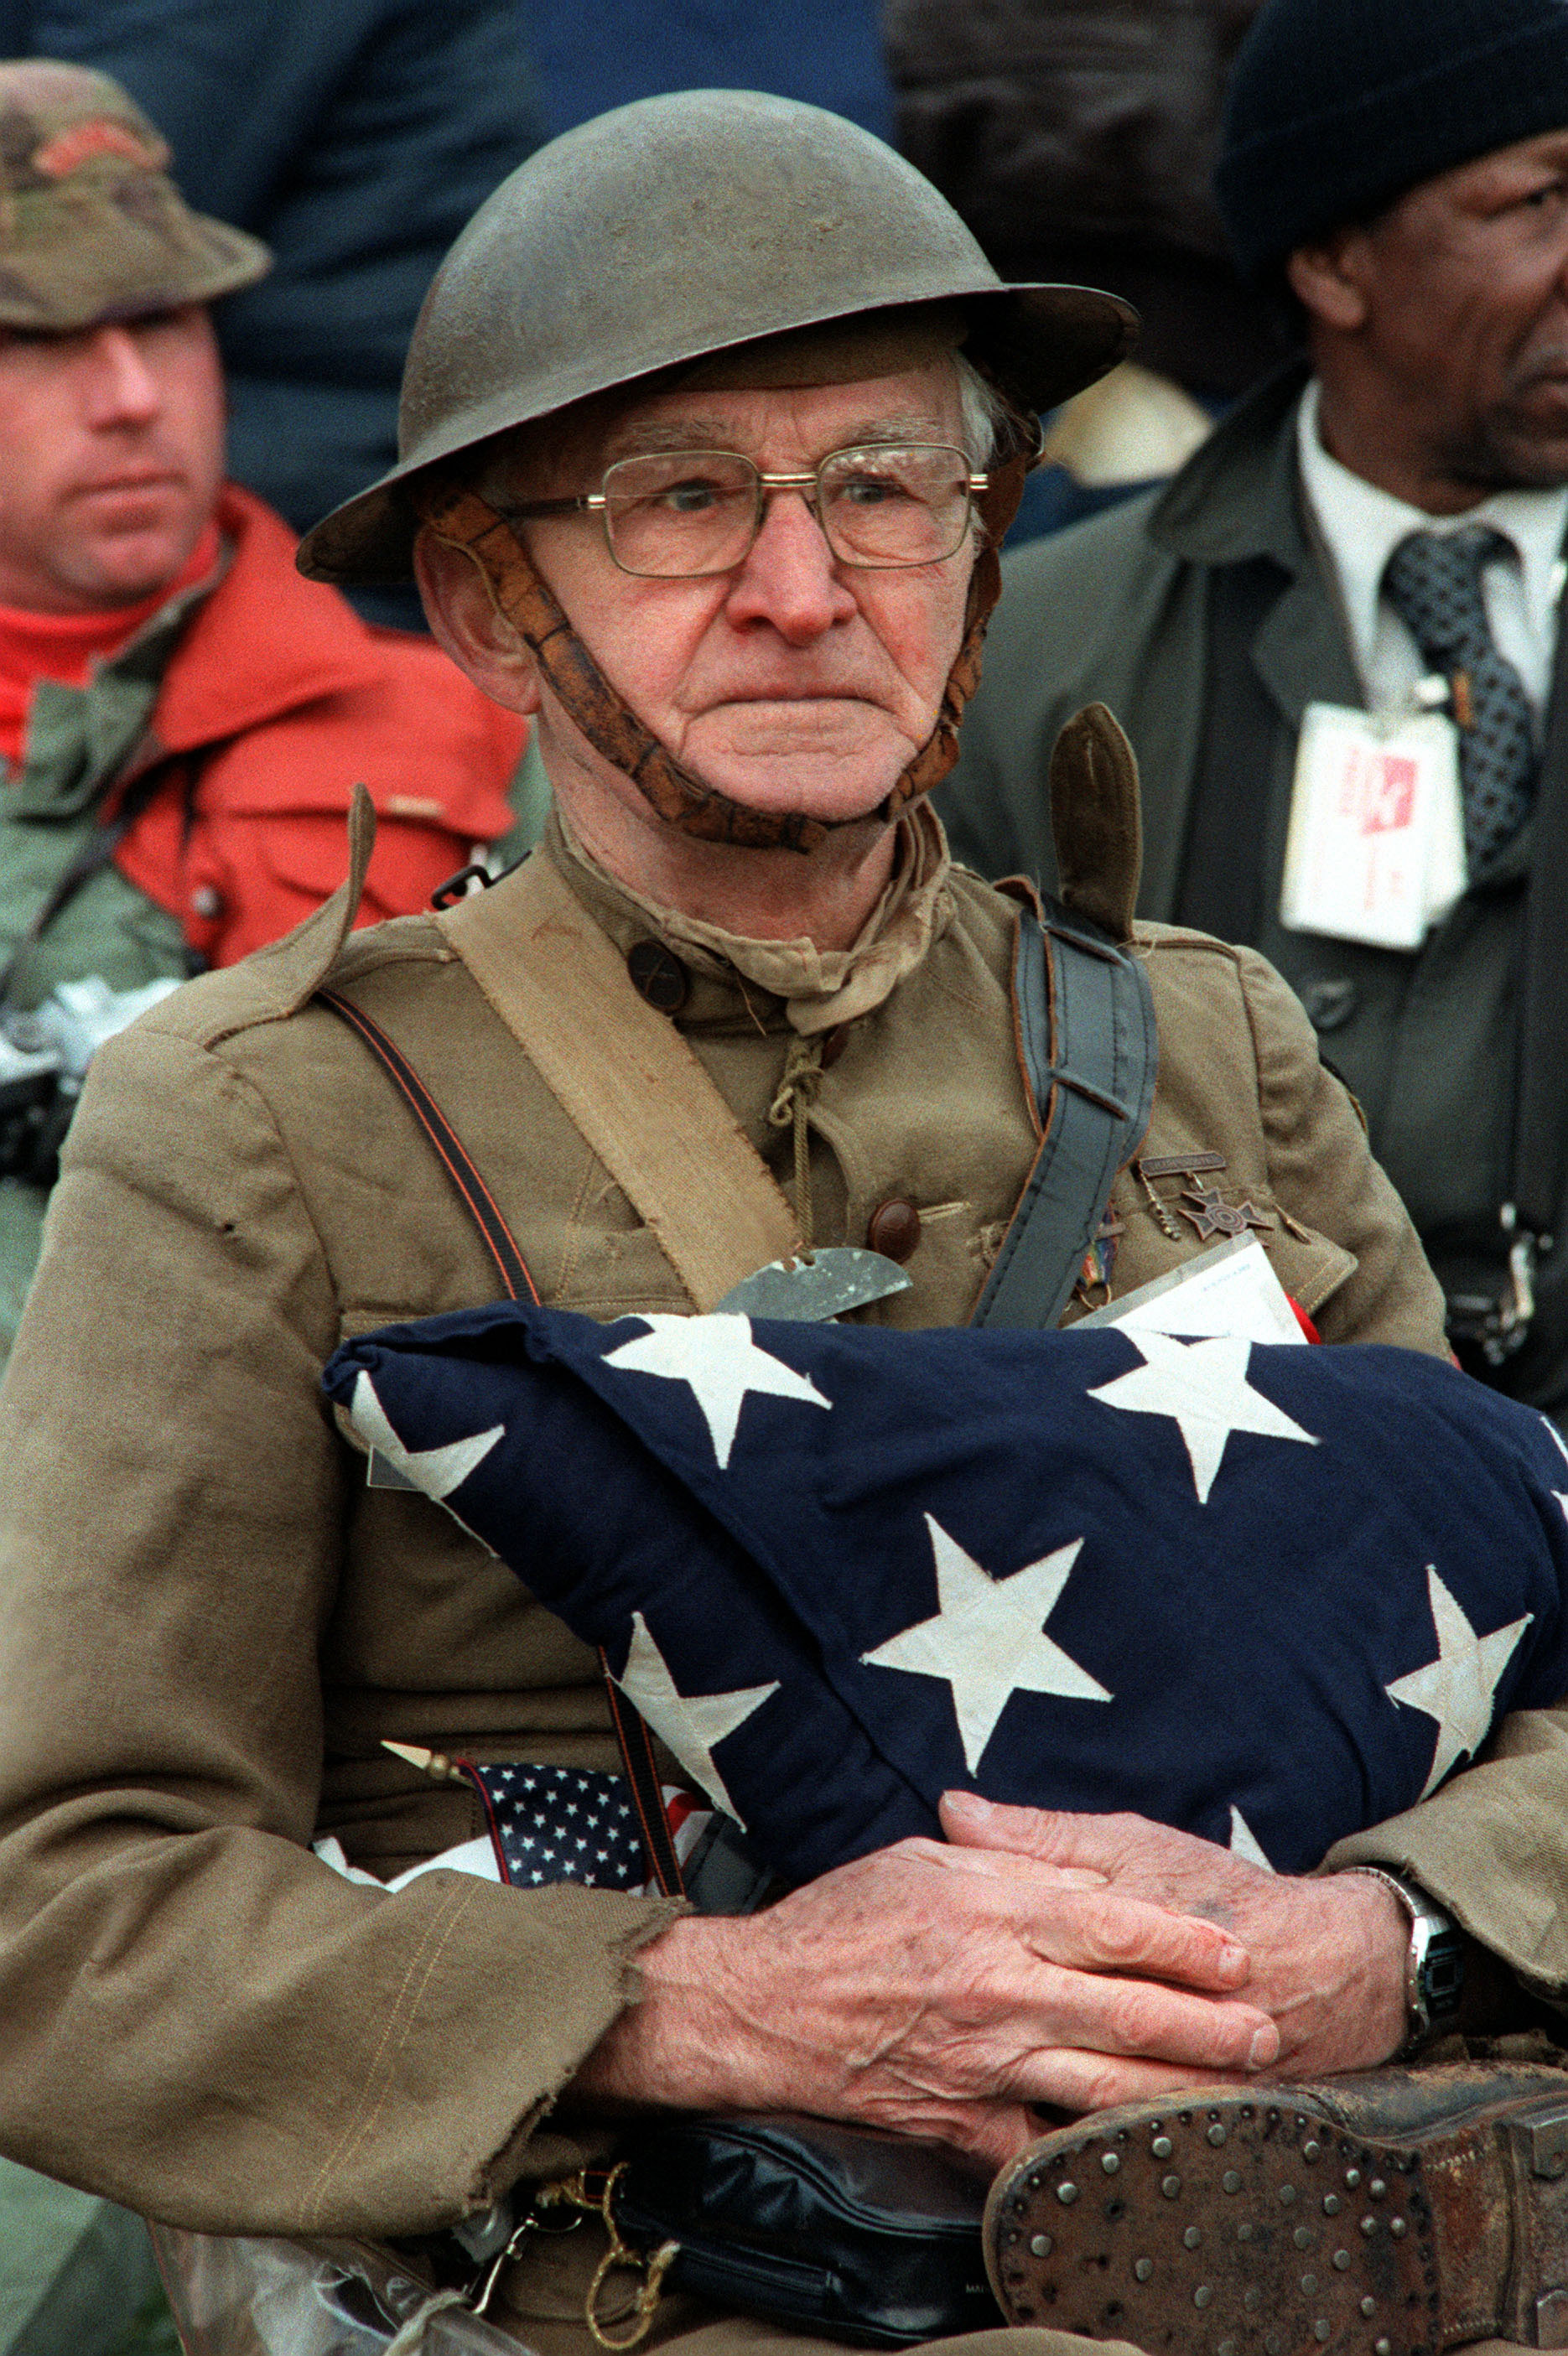
\includegraphics[scale=0.2]{veteran.jpg}
              }
            \end{center}
          \end{minipage}
      \end{columns}
    }
  \end{frame}

  \begin{frame}{Les anniversaires}
    En groupes de 3 ou 4, demandez à votre tour l'anniversaire de chaque personne.
    Par exemple: \\
    \tinygloss{In groups of 3 or 4, take turns asking each person when their birthday is.
    For example:}
    \begin{columns}
      \column{0.5\textwidth}
        \begin{description}
          \item[E1:] Ton anniversaire, c'est quel jour?
          \item[] \tinygloss{Your birthday, it's what day?}
          \item[E2:] C'est le 30 septembre.
          \item[] \tinygloss{It's September 30th.}
        \end{description}
      \column{0.5\textwidth}
        \begin{center}
          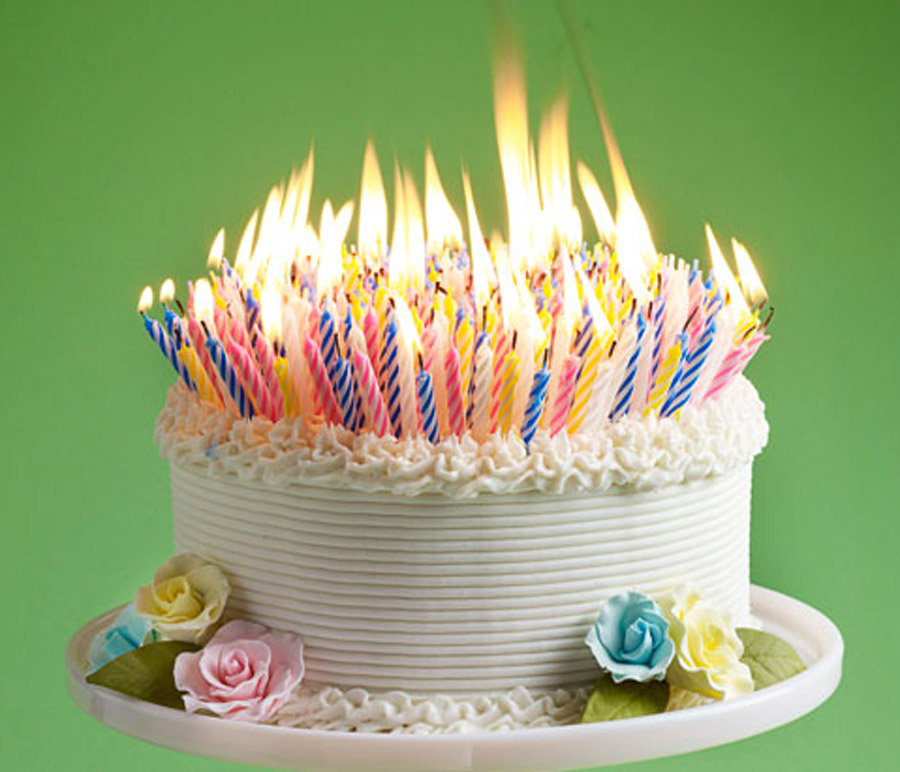
\includegraphics[scale=0.14]{anniversaire.jpg}
        \end{center}
    \end{columns}
  \end{frame}
  % Follow by asking who has a group member with birthdays on certain days or in
  % certain months.

  \begin{frame}{Cours de mathématiques}
    Avec un/e partenaire, posez à votre tour des problèmes de maths simples en utilisant l'addition (\lexi{plus}) et la soustraction (\lexi{moins}).
    Par exemple: \\
    \tinygloss{Work with a partner and take turns giving each other simple math problems using addition (\lexi{plus}) or subtraction (\lexi{moins}).
    For example:}
    \begin{columns}
      \column{0.5\textwidth}
        \begin{description}
          \item[E1:] 10 plus 2, ça fait combien?
          \item[] \tinygloss{10 plus 2, that makes how many?}
          \item[E2:] Ça fait 12.
          \item[] \tinygloss{That makes 12.}
        \end{description}
      \column{0.5\textwidth}
        \begin{center}
          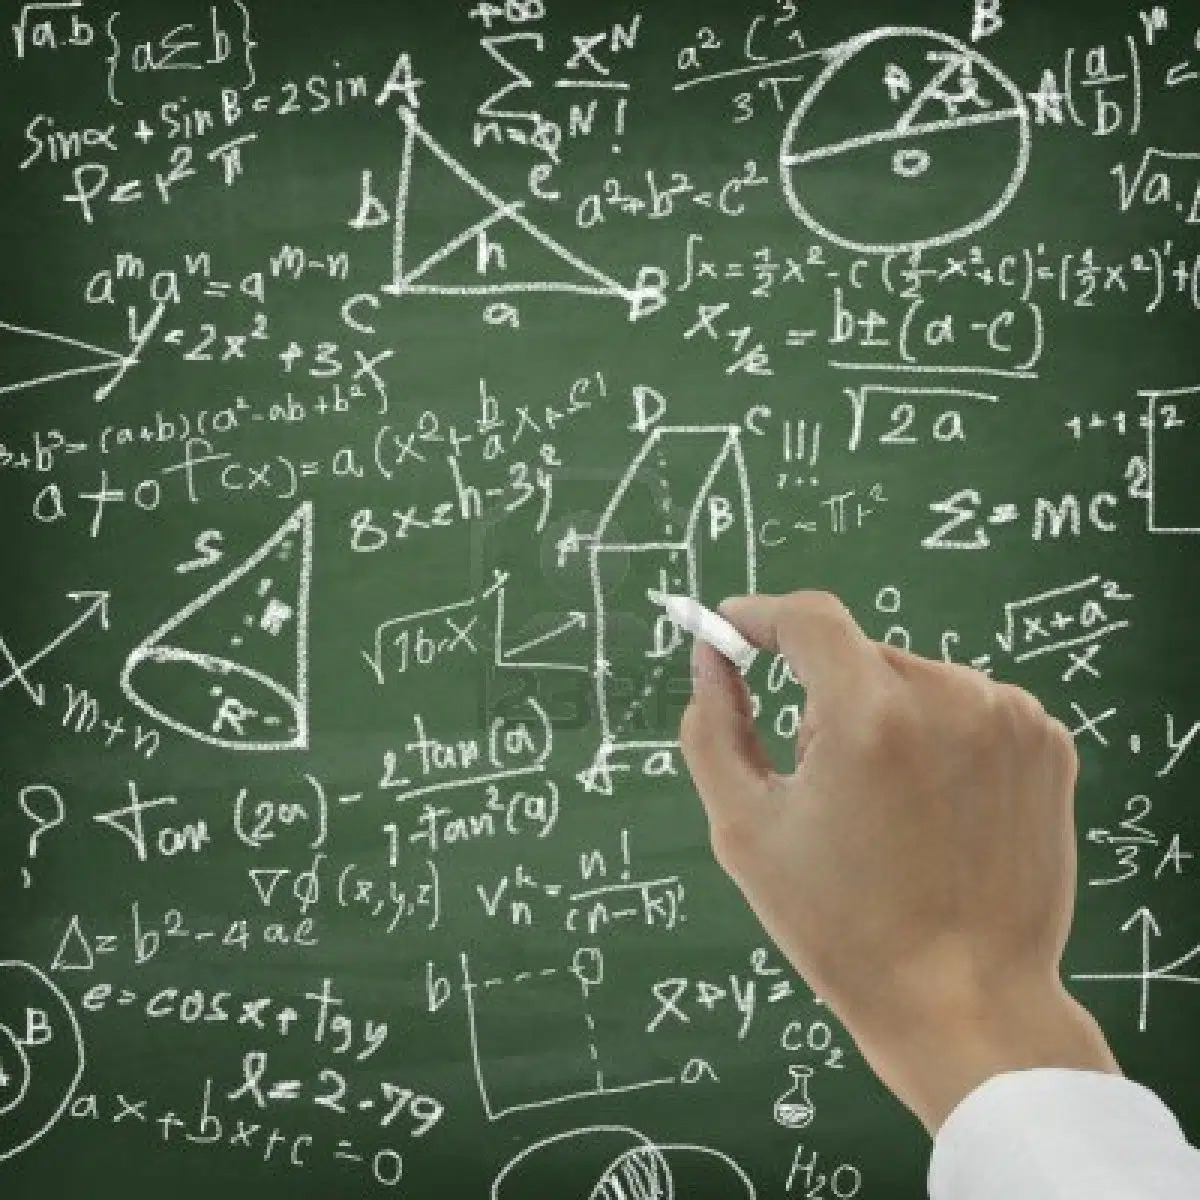
\includegraphics[scale=0.1]{maths.jpg}
        \end{center}
    \end{columns}
  \end{frame}

  \begin{frame}{}
    \begin{center}
      \Large Questions?
    \end{center}
  \end{frame}
\end{document}
